\documentclass[UTF8,a4paper,11pt,fontset=fandol]{ctexart}
\usepackage[margin=23mm]{geometry}
\usepackage{amsmath,amssymb,booktabs,longtable,graphicx,float,fancyhdr,xcolor,needspace}
\usepackage{xurl}
\usepackage[unicode,colorlinks=true,linkcolor=black,urlcolor=blue]{hyperref}
\definecolor{accent}{HTML}{155574}
\pagestyle{fancy}
\fancyhf{}
\fancyhead[L]{\small 数学建模训练论文}
\fancyhead[R]{\small 待人工审阅}
\fancyfoot[C]{\thepage}
\setlength{\headheight}{15pt}
\setlength{\parskip}{0.35em}
\setlength{\emergencystretch}{3em}
\title{\bfseries 基于时间顺序验证的日需求预测与基线比较}
\author{}
\date{}
\begin{document}
\maketitle
\vspace{-2.4em}
\begin{center}\small\color{accent}训练草稿：计算已核验，建模解释、引用及赛事格式仍需队员审阅\end{center}
\begin{abstract}
针对日需求预测问题，使用 112 个连续日观测，设置最终留出测试集，并仅在测试集之前的数据上开展扩展窗口验证。训练期比较后选定 趋势与周周期模型 模型。最终测试均方根误差为 2.108，周朴素基线为 4.321，相对变化为 51.21\%。之后用全部观测重新拟合，未来预测期合计需求为 886.64。结果为点预测，其适用范围限于教学数据及已声明假设。
\end{abstract}
\noindent\textbf{关键词：}时间顺序验证；需求预测；周周期；基线比较

\section{问题分析与数据来源}
本案例数据由固定随机种子的趋势、周周期和随机扰动构造，仅用于教学与软件评测；生成程序保存在 generate\_data.py。
\begin{description}

\item[Q1] 比较周朴素、线性趋势、趋势加周周期模型，并用训练期验证选择方法。

\item[Q2] 在留出测试集评价预测误差，再用全部已观测数据拟合并预测未来需求。

\end{description}

\section{模型假设与符号}
\begin{enumerate}

\item 日需求具有可由候选模型近似的趋势或周周期。

\item 观测日期连续且单位一致，预测时只能使用预测起点之前已知的信息。

\item 当前候选模型未纳入节假日、价格与结构突变等外部因素。

\end{enumerate}
\begin{longtable}{p{.16\textwidth}p{.46\textwidth}p{.20\textwidth}}
\toprule 符号 & 含义 & 单位 \\ \midrule

t & 自起始日期起的日序号 & 日 \\

y\_t & 日观测值 & 需求单位/日 \\

\bottomrule
\end{longtable}

\section{模型建立与求解方法}
仅在最终测试集之前的数据上进行扩展窗口验证，按平均 RMSE 选择模型；测试集只评价一次。

\begin{equation}
\widehat y_t=\beta_0+\beta_1t
\end{equation}

\begin{equation}
\widehat y_t=\beta_0+\beta_1t+\beta_2\sin(2\pi t/7)+\beta_3\cos(2\pi t/7)
\end{equation}

\begin{equation}
\operatorname{RMSE}=\sqrt{N^{-1}\sum_t(y_t-\widehat y_t)^2}
\end{equation}

\noindent\textbf{基线方案：}同星期朴素预测（仅使用预测起点之前最后一周的观测）。


\section{候选模型与训练期选择}
候选方法包含同星期朴素模型、线性趋势模型及趋势加周周期模型。参数通过最小二乘估计[numpy\_lstsq]。所有验证窗口均位于最终测试期之前；根据训练期平均验证误差选定 趋势与周周期模型，比较结果列于模型表。最终测试集不参与候选方法选择。

\section{独立测试与未来预测}
最终留出样本数为 14，所选方法的均方根误差为 2.108，平均绝对误差为 1.737。周朴素基线的均方根误差为 4.321，相对变化为 51.21\%。完成评价后，使用全部已观测数据重新拟合，未来预测期合计需求为 886.64。预测结果没有附加未经校准的置信区间。


\section{计算结果与图表}
所有数值均读取同一次实验记录；表中的不可用项保留其原始状态。

\Needspace{7\baselineskip}
\subsection*{留出测试集逐日比较}
{\small
\begin{longtable}{llll}
\toprule
日期 & 观测值 & 预测值 & 基线值 \\ 
\midrule\endhead

2026-04-09 & 121.05 & 121.74 & 121.47 \\ 

2026-04-10 & 133.69 & 132.3 & 130.7 \\ 

2026-04-11 & 133.68 & 135.02 & 131.57 \\ 

2026-04-12 & 125.7 & 128.08 & 124.39 \\ 

2026-04-13 & 118.6 & 116.95 & 112.43 \\ 

2026-04-14 & 109.88 & 110.26 & 109.17 \\ 

2026-04-15 & 113 & 113.28 & 108.07 \\ 

2026-04-16 & 122.57 & 123.97 & 121.47 \\ 

2026-04-17 & 136.85 & 134.54 & 130.7 \\ 

2026-04-18 & 137.52 & 137.25 & 131.57 \\ 

2026-04-19 & 126.44 & 130.31 & 124.39 \\ 

2026-04-20 & 121.09 & 119.19 & 112.43 \\ 

2026-04-21 & 108.13 & 112.49 & 109.17 \\ 

2026-04-22 & 113.42 & 115.51 & 108.07 \\ 

\bottomrule
\end{longtable}}

\Needspace{7\baselineskip}
\subsection*{未来逐日点预测}
{\small
\begin{longtable}{ll}
\toprule
日期 & 预测值 \\ 
\midrule\endhead

2026-04-23 & 125.94 \\ 

2026-04-24 & 136.53 \\ 

2026-04-25 & 139.22 \\ 

2026-04-26 & 132.21 \\ 

2026-04-27 & 121.03 \\ 

2026-04-28 & 114.32 \\ 

2026-04-29 & 117.38 \\ 

\bottomrule
\end{longtable}}

\Needspace{7\baselineskip}
\subsection*{训练期扩展窗口比较}
{\small
\begin{longtable}{ll}
\toprule
候选模型 & 验证 RMSE \\ 
\midrule\endhead

周朴素模型 & 5.3841 \\ 

线性趋势模型 & 10.103 \\ 

趋势与周周期模型 & 2.8878 \\ 

\bottomrule
\end{longtable}}


\begin{figure}[H]
\centering
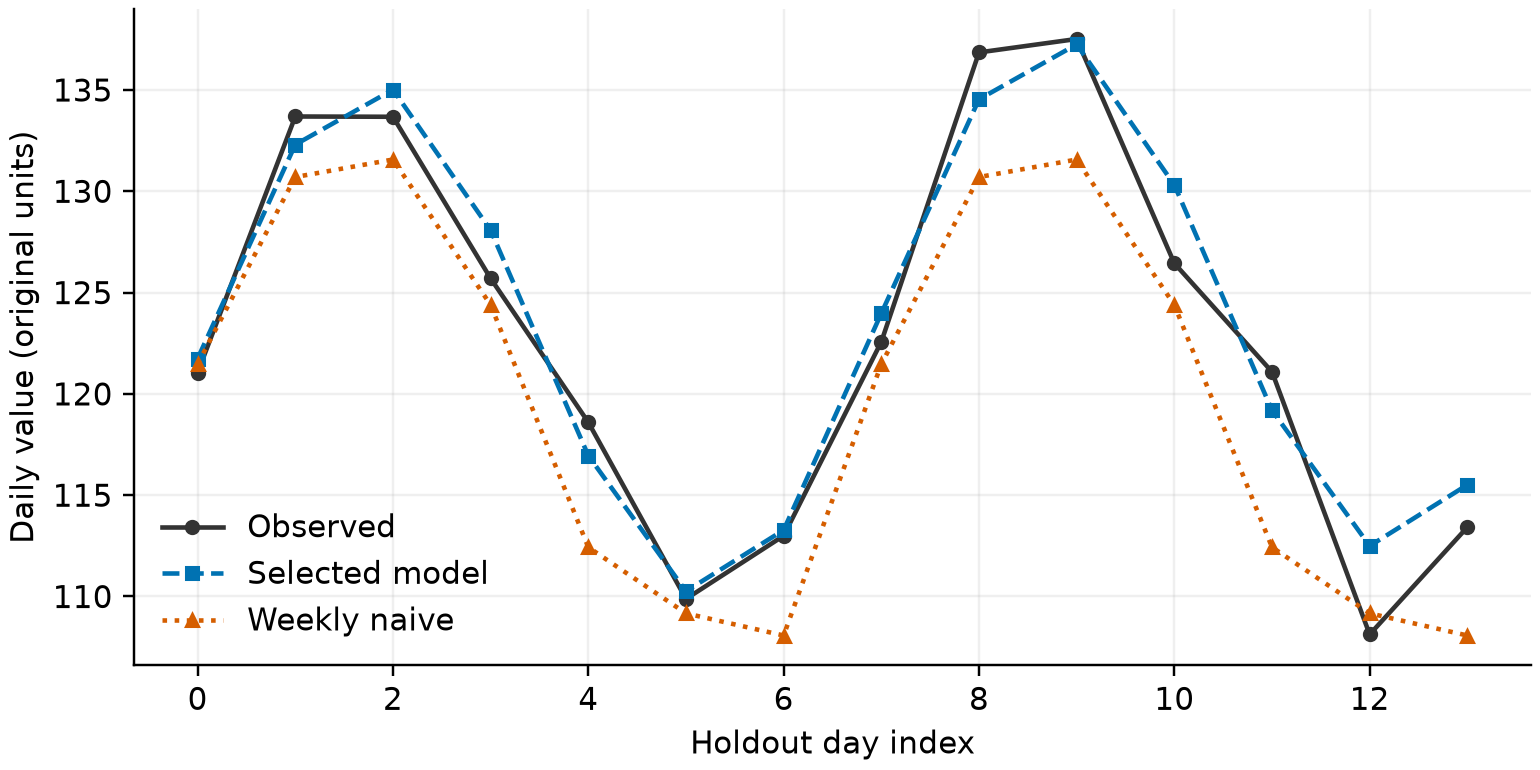
\includegraphics[width=.91\textwidth]{../figures/holdout.png}
\caption{最终留出测试集上的实际值、所选模型与周朴素基线预测。}
\end{figure}

\begin{figure}[H]
\centering
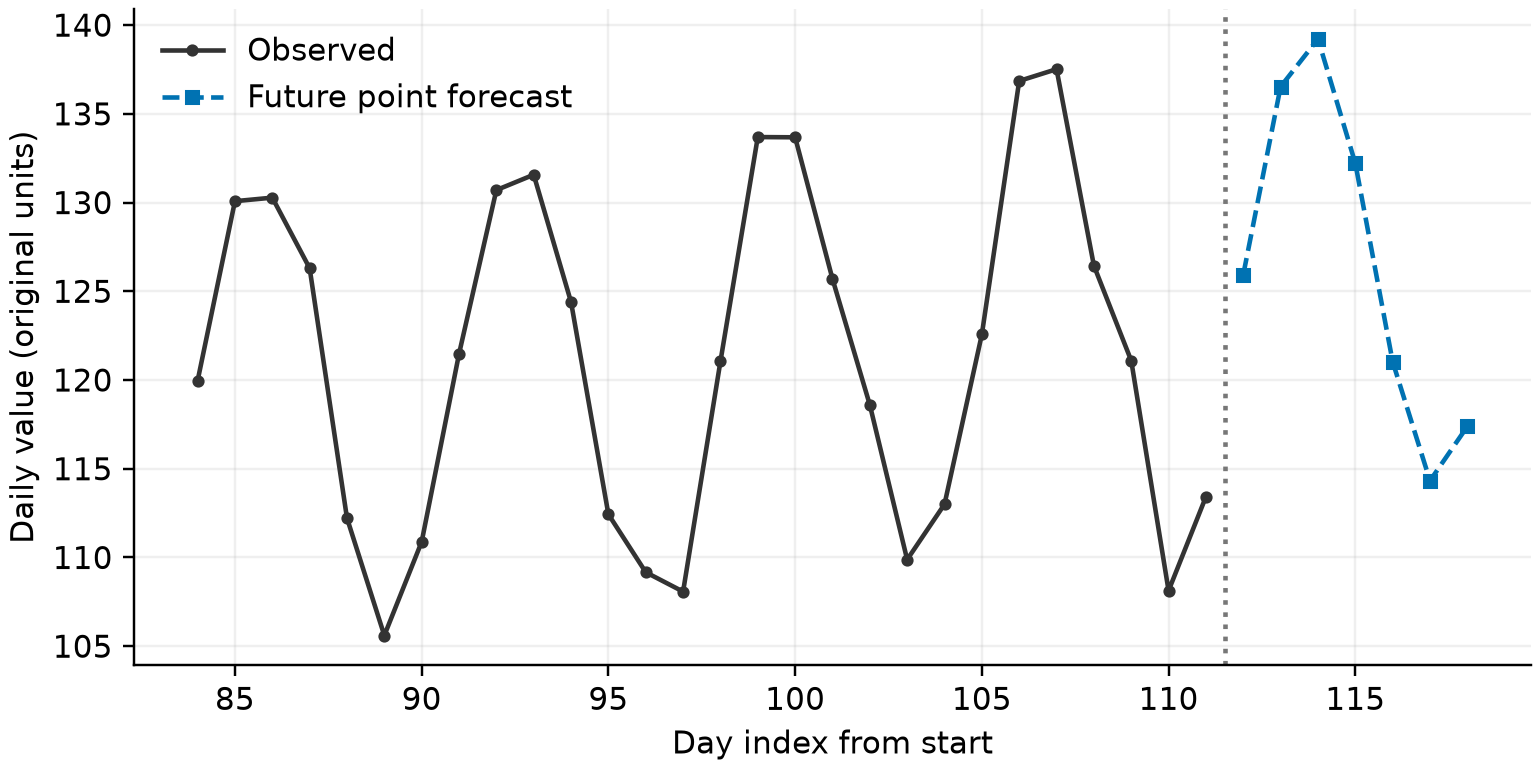
\includegraphics[width=.91\textwidth]{../figures/forecast.png}
\caption{使用全部已观测数据重新拟合后的未来点预测；竖线右侧为外推区间。}
\end{figure}


\section{检验、局限与改进方向}
本次自动核验覆盖了已编码的数值条件。自动核验通过不等价于题意解释已经充分，队员仍需对照原题审阅假设与结论。
\begin{itemize}

\item 候选模型仅含周周期和线性趋势，结构突变会影响外推。

\item 结果是点预测；本案例未估计经校准的预测区间。

\end{itemize}

\section*{参考来源}

\begin{description}

\item[numpy\_lstsq] NumPy 官方文档：最小二乘求解 numpy.linalg.lstsq. \url{https://numpy.org/doc/stable/reference/generated/numpy.linalg.lstsq.html}. 核验状态：opened\_by\_agent.

\end{description}

\section*{复现与 AI 使用说明}
数据来源、程序版本和输入摘要见工作区中的 provenance.json；运行命令见复现说明。
本案例使用已声明的训练数据，结论仅用于演示建模过程。
实际 AI 工具使用、人工修改及核验记录保存在 ai\_usage.jsonl 中，由队员据实补充后按赛事要求整理。
\end{document}